\documentclass[conference,a4paper]{IEEEtran}
\IEEEoverridecommandlockouts
% The preceding line is only needed to identify funding in the first footnote.
\usepackage{cite}
\usepackage{amsmath,amssymb,amsfonts}
\usepackage{graphicx}
\usepackage{textcomp}
\usepackage{xcolor}
\usepackage{booktabs}
\usepackage{url}
\usepackage{tikz}
\usetikzlibrary{arrows.meta,decorations.pathreplacing,calc,positioning}

% ICEIC 2027 format: 2-6 pages, two-column A4, font >= 10 pt. Fig. 1 is fig_overview_res.tex (TikZ);
% figures/res_forest.pdf and res_general.pdf come from scripts/fig_paper.py and figures/res_qual.pdf
% from scripts/qual_frames.py + scripts/fig_qual.py of the code release.

\begin{document}

\title{When to Replan and How Much to Correct:\\
Residual Reinforcement Learning for Disturbance\\
Recovery in Vision-Language-Action Policies
\thanks{This work was supported by grants from the Institute of Information \&
Communications Technology Planning \& Evaluation (IITP) funded by the Korea
government (MSIT) [Artificial Intelligence Research Hub Project,
No.~\mbox{RS-2024-00457882}; Artificial Intelligence Graduate School Program at
Korea University, No.~\mbox{RS-2019-II190079}; Information Technology Research
Center (ITRC) program, No.~\mbox{IITP-2026-RS-2024-00436857}] and by a grant
from the National Research Foundation of Korea (NRF) funded by the Korea
government (MSIT) (No.~\mbox{RS-2023-00212498}).}
}

\author{\IEEEauthorblockN{Chang-Hoon Ji}
\IEEEauthorblockA{\textit{Department of Artificial Intelligence} \\
\textit{Korea University}\\
Seoul, Republic of Korea \\
ckdgns0611@korea.ac.kr}
\and
\IEEEauthorblockN{Tae-Eui Kam}
\IEEEauthorblockA{\textit{Department of Artificial Intelligence} \\
\textit{Korea University}\\
Seoul, Republic of Korea \\
kamte@korea.ac.kr}
}

\maketitle

% No math, symbols, or footnotes in the abstract (IEEE rule).
\begin{abstract}
Vision-language-action policies execute predicted action chunks open loop, so after an object is suddenly displaced, the robot follows a plan made for the old scene. On LIBERO-10, teleporting the target object by 4 to 6 cm, mostly as the gripper approaches, cuts the pi0.5 policy's success from 95 to 65 percent. Under one paired protocol, simple inference-time levers (replan frequency, integration steps, chunk selection) recover little. More computation at the next scheduled query recovers nothing measurable, whereas moving the query to the event with a learned camera-frame detector recovers about three points without adding policy queries per episode. Correcting the actions recovers more. A fixed-rule shift toward the estimated displacement gains about six points. An event-gated residual, cloned from a scripted shift on privileged state, refined with reinforcement learning as lightweight post-training and distilled into a vision-only student, raises success on initial states not used for training from 62.2 to 71.8 percent (gain 9.6 points, 95 percent interval 5.8 to 13.4; 11.2 on all 500 episodes, 8.3 with displacements twice as large), with no measurable change in undisturbed success.
\end{abstract}

\begin{IEEEkeywords}
vision-language-action models, post-training, residual reinforcement
learning, action chunking, event-triggered replanning, disturbance detection
\end{IEEEkeywords}

% =====================================================================
\section{Introduction}
% =====================================================================

Vision-language-action (VLA) models have become a standard recipe for
language-conditioned manipulation~\cite{kim2024openvla,black2024pi0,pi05}.
Most now predict \emph{action chunks}~\cite{zhao2023act,chi2025diffusion}:
one query of the model yields a short sequence of $H$ actions, of which the robot
executes a prefix of $h$ steps before the model is queried again. Chunking smooths motion and amortizes the backbone's cost but makes the
controller open loop between queries. If the scene changes
inside a chunk, the robot executes actions planned for the old scene
until the chunk is spent, and the next query sees a configuration the training data
rarely contains.

% =====================================================================
% fig_overview_res.tex -- Fig. 1 of the residual-recovery paper (TikZ).
% Requires in the preamble:
%   \usepackage{tikz}
%   \usetikzlibrary{arrows.meta,decorations.pathreplacing,calc,positioning}
% =====================================================================
\begin{figure*}[t]
\centering
\definecolor{cexec}{RGB}{0,114,178}
\definecolor{cevent}{RGB}{213,94,0}
\definecolor{ctrig}{RGB}{230,159,0}
\definecolor{cres}{RGB}{0,158,115}
\definecolor{cvla}{RGB}{86,180,233}
\definecolor{creg}{RGB}{204,121,167}
\resizebox{0.97\textwidth}{!}{%
\begin{tikzpicture}[
  >={Stealth[length=4pt,width=3pt]},
  font=\footnotesize,
  cell/.style={draw=black!55, line width=0.3pt, minimum width=0.30cm,
               minimum height=0.30cm, inner sep=0pt, outer sep=0pt},
  exe/.style={cell, fill=cexec!55},
  old/.style={cell, fill=cexec!18,
    path picture={\draw[black!45, line width=0.3pt]
      (path picture bounding box.south west) --
      (path picture bounding box.north east);}},
  cor/.style={cell, fill=cres!45},
  qry/.style={draw=ctrig!70!black, fill=ctrig!60, line width=0.3pt,
              rounded corners=1pt, minimum height=0.26cm, minimum width=0.16cm,
              inner sep=0pt},
  box/.style={draw=black!60, line width=0.4pt, rounded corners=2pt,
              align=center, inner sep=2.5pt, font=\footnotesize},
  lbl/.style={font=\footnotesize},
  flow/.style={->, line width=0.5pt}
]

% ------------------------------------------------------------------
% Panel (a): three reactions to a displacement inside a chunk
% ------------------------------------------------------------------
\def\w{0.30}      % cm per control step
\def\xo{2.55}     % x of the first action of chunk i
\def\td{4}        % displacement happens after action 4 of chunk i

% row (i): scheduled replanning (baseline)
\def\yA{0}
\node[lbl, anchor=east, align=right] at (\xo-0.1,\yA)
  {(i) scheduled replan\\[-1pt] (baseline)};
\foreach \t in {0,...,3} \node[exe] at ({\xo+(\t+0.5)*\w},\yA) {};
\foreach \t in {4,...,9} \node[old] at ({\xo+(\t+0.5)*\w},\yA) {};
\node[qry] at ({\xo+10*\w},\yA) {};
\foreach \t in {10,...,16} \node[exe] at ({\xo+(\t+0.5)*\w},\yA) {};
\node[lbl, anchor=west] at ({\xo+17*\w+0.1},\yA) {stale chunk runs out};

% row (ii): event-triggered replanning
\def\yB{-0.62}
\node[lbl, anchor=east, align=right] at (\xo-0.1,\yB)
  {(ii) replan at the\\[-1pt] event (detector)};
\foreach \t in {0,...,3} \node[exe] at ({\xo+(\t+0.5)*\w},\yB) {};
\node[old] at ({\xo+4.5*\w},\yB) {};
\node[qry] at ({\xo+5*\w},\yB) {};
\foreach \t in {5,...,16} \node[exe] at ({\xo+(\t+0.5)*\w},\yB) {};
\node[qry] at ({\xo+15*\w},\yB) {};
\node[lbl, anchor=west] at ({\xo+17*\w+0.1},\yB) {$+2.8$ pts, $1.00\times$ cost};

% row (iii): event-triggered replanning + residual correction
\def\yC{-1.24}
\node[lbl, anchor=east, align=right] at (\xo-0.1,\yC)
  {(iii) + residual\\[-1pt] correction};
\foreach \t in {0,...,3} \node[exe] at ({\xo+(\t+0.5)*\w},\yC) {};
\node[old] at ({\xo+4.5*\w},\yC) {};
\node[qry] at ({\xo+5*\w},\yC) {};
\foreach \t in {5,...,16} \node[cor] at ({\xo+(\t+0.5)*\w},\yC) {};
\node[qry] at ({\xo+15*\w},\yC) {};
\node[lbl, anchor=west] at ({\xo+17*\w+0.1},\yC) {$+9.6$ pts, vision only};

% displacement marker
\draw[cevent, line width=0.6pt] ({\xo+\td*\w},\yA+0.25) -- ({\xo+\td*\w},\yC-0.25);
\node[lbl, cevent, above] at ({\xo+\td*\w},\yA+0.24) {object displaced 4--6\,cm};
\draw[decorate, decoration={brace, amplitude=2.5pt, mirror}, line width=0.4pt, cres!80!black]
  ({\xo+5*\w},\yC-0.22) -- node[lbl, below=1.5pt, cres!80!black]
  {$a_t\leftarrow a_t+\Delta$ for the next 6 queries} ({\xo+17*\w},\yC-0.22);

% time axis
\def\yT{-2.05}
\draw[->, line width=0.4pt] (\xo,\yT) -- ({\xo+17*\w+0.3},\yT);
\foreach \t in {0,5,10,15} {
  \draw[line width=0.3pt] ({\xo+\t*\w},\yT) -- ({\xo+\t*\w},\yT-0.06);
  \node[lbl, below] at ({\xo+\t*\w},\yT-0.03) {\t};}
\node[lbl, anchor=west] at ({\xo+17*\w+0.35},\yT) {control step};

% legend
\node[exe] at (0.35,-2.62) {};  \node[lbl, anchor=west] at (0.55,-2.62) {executed action};
\node[old] at (2.75,-2.62) {};  \node[lbl, anchor=west] at (2.95,-2.62) {planned before the event};
\node[cor] at (6.45,-2.62) {};  \node[lbl, anchor=west] at (6.65,-2.62) {corrected};
\node[qry, minimum width=0.16cm] at (8.15,-2.62) {}; \node[lbl, anchor=west] at (8.35,-2.62) {policy query};

\node[font=\footnotesize] at (4.6,-3.1)
  {(a) Reactions to a displacement inside a chunk ($H{=}h{=}10$)};

% ------------------------------------------------------------------
% Panel (b): vision-only pipeline and its training
% ------------------------------------------------------------------
\def\xb{11.0}

\node[box, fill=ctrig!15, draw=ctrig!70!black, minimum width=1.9cm] (det) at (\xb+1.7,0.05)
  {disturbance detector\\ CNN, every step};
\node[box, fill=cvla!15, draw=cvla!70!black, minimum width=1.9cm] (vla) at (\xb+5.9,0.05)
  {$\pi_{0.5}$ policy\\ query $\rightarrow$ chunk $\mathbf{A}$};
\node[box, fill=creg!15, draw=creg!70!black, minimum width=1.9cm] (reg) at (\xb+1.7,-1.25)
  {displacement regressor\\ CNN on the event frames};
\node[box, fill=cres!15, draw=cres!70!black, minimum width=1.9cm] (res) at (\xb+5.9,-1.25)
  {residual MLP\\ $\Delta=\mathbf{s}\odot\tanh u(x)$};
\node[circle, draw=black!60, line width=0.4pt, inner sep=0pt, minimum size=0.26cm, font=\scriptsize] (sum)
  at (\xb+7.75,-0.6) {$+$};
\node[box, fill=black!5, minimum height=1.9cm, minimum width=0.5cm, inner sep=1pt] (rob) at (\xb+8.45,-0.6)
  {\rotatebox{90}{robot}};

\node[lbl, align=center] (obsin) at (\xb+1.7,0.92) {frames $o_{t-1},o_t$ (2 cameras), $a_{t-1}$, end-effector motion};
\node[lbl] (vlain) at (\xb+5.9,0.92) {$o_t,\ell$};
\draw[flow] (obsin.south) -- (det.north);
\draw[flow] (vlain.south) -- (vla.north);
\draw[flow] (det) -- node[lbl, above, inner sep=1pt] {replan} (vla);
\draw[flow] (det) -- node[lbl, right] {event frames} (reg);
\draw[flow] (reg) -- node[lbl, above] {$\hat d$} (res);
\draw[flow] (vla.east) -| (sum.north);
\draw[flow] (res.east) -| (sum.south);
\draw[flow] (sum) -- (rob);
\node[lbl, anchor=north, align=center] at (\xb+4.35,-1.7)
  {$x$: proprio, chunk statistics, $\hat d$, queries since the event, task};

% training strip
\node[box, fill=white, inner sep=1.5pt, align=left] (train)
  at (\xb+4.35,-2.5)
  {training in simulation: scripted shift $0.5\,d$ $\rightarrow$ BC $\rightarrow$ PPO teacher (privileged $d$)\\[-1pt]
   $\rightarrow$ DAgger ($\beta=1,0.5,0$) $\rightarrow$ vision-only student; detector, regressor: supervised};

\node[font=\footnotesize] at (\xb+4.35,-3.1) {(b) Vision-only system: when to replan, how much to correct};

\end{tikzpicture}%
}
\caption{Overview. (a) A chunked policy that is queried every $h$ actions
cannot react to a displacement until the current chunk is spent (i).
A learned detector interrupts the chunk and replans at the event (ii), and a residual policy adds a small correction $\Delta$ to every action of the
following queries (iii). (b) All three learned modules use only camera
frames, actions, proprioception and the task; the
$\pi_{0.5}$ weights are not updated. Gains: held-out episodes, as in Fig.~\ref{fig:forest}.}
\label{fig:overview}
\end{figure*}


How large is this cost, and what recovers it? We study the question with the
official $\pi_{0.5}$ checkpoint for LIBERO~\cite{pi05,liu2023libero} under
a controlled disturbance: when the open gripper first comes within 12\,cm of
the object it is approaching (or at a random step if it has not by then), the object is teleported 4--6\,cm horizontally,
which cuts success on LIBERO-10 from 95.4\% to 64.7\%. Tracking the object
(Section~\ref{sec:diag}) shows that the policy often first closes the gripper nearer the \emph{old} position.

Recent work offers several responses. Adaptive-inference methods decide
when to replan, how much to compute per query, or which of several sampled
chunks to keep~\cite{liang2026aac,pan2026corrector,chun2025dasip,liu2025bid}; runtime
monitors detect execution failures~\cite{agia2024sentinel,xu2025faildetect,gu2025safe};
and residual reinforcement learning (RL) learns corrections on top of a fixed policy~\cite{yuan2025decorator,xiao2025pld}.
They are evaluated on different tasks and disturbances; a concurrent benchmark of mid-execution changes such as target relocation finds, for four of its 14 policies including $\pi_{0.5}$, that varying the query cadence does not close the gap, but tests no event-triggered replanning or action correction~\cite{zhang2026liberomax}. We test simple versions of each response under one protocol. Moving the query to the event helps by only about three points, and the new chunk seems to aim only partly at the new position; correcting the actions recovers more: about six of the 31 lost points with a fixed rule and about ten with a detector-gated residual policy trained with RL as lightweight post-training around the VLA (Fig.~\ref{fig:overview}).

Our contributions are:
\begin{itemize}
  \item a paired evaluation on LIBERO-10 in which every variant faces the same seeded mid-execution displacement
        and is compared with the mean of seven sampling-noise draws of the base policy
        (complementing studies that perturb the setup before execution~\cite{fei2025liberoplus}
        or the robot's actions during it~\cite{guo2026robustvla,gao2026ogpo}), with a diagnosis of the failure;
  \item under it, a comparison showing that simple inference levers do not
        recover the loss and that moving the query to the event recovers about three of the 31 points while more computation at the next scheduled query recovers nothing measurable, with a learned per-step detector
        that recognizes 87--90\% of displacements on held-out initial states within three control steps;
  \item an event-gated residual recovery policy, trained as a privileged teacher by behavior cloning (BC) of a scripted
        shift followed by proximal policy optimization (PPO) and distilled into
        a vision-only student, that adds 3.9 points over a fixed-rule shift on held-out initial states (4.7 on all 500),
        still gains with displacements twice as large and causes no measurable change in
        undisturbed success.\footnote{Code, trained modules and per-episode results:\newline \url{https://github.com/BitAdventurer/VLA-Disturbance-Recovery}}
\end{itemize}

% =====================================================================
\section{Related Work}\label{sec:related}
% =====================================================================

\noindent\textbf{Adaptive chunk execution.}
AAC sets the executed prefix of a chunk from the entropy of sampled
chunks~\cite{liang2026aac}, bidirectional decoding selects among chunks
resampled at every step~\cite{liu2025bid}, RTC inpaints the next chunk
while the current one executes~\cite{black2025rtc}, DVAC executes the
low-variance prefix of a chunk and replans before its high-variance
actions~\cite{feng2026dvac}, and DA-SIP chooses the number of integration
steps per query with a difficulty classifier~\cite{chun2025dasip}. They balance reactivity, consistency and compute but detect no events. VLA-Corrector~\cite{pan2026corrector} does: it truncates the chunk when visual latents drift from a learned prediction and replans with gradient guidance, but adds no correction policy and tests displacement only on hardware.

\noindent\textbf{Runtime monitoring.}
Sentinel~\cite{agia2024sentinel}, FAIL-Detect~\cite{xu2025faildetect} and SAFE~\cite{gu2025safe} flag failures or halt the policy based on action consistency and task progress, on sequential out-of-distribution tests and on VLA features, respectively. Like VLA-Corrector, we use detection to \emph{act}, here on one external event.

\noindent\textbf{Correcting a fixed policy's actions.}
Residual RL~\cite{johannink2019residual} refines imitation-learned policies~\cite{yuan2025decorator,ankile2024resip} and a
frozen $\pi_0$, with the corrections then distilled into the VLA~\cite{xiao2025pld}, and latent-noise RL steers $\pi_0$ without changing its weights~\cite{wagenmaker2025dsrl}. Other work post-trains the VLA itself with online
RL~\cite{chen2025conrft,guo2025irevla}, which has been shown to help when an
object is moved mid-episode~\cite{liu2025rl4vla}, or with offline RL to recover from errors~\cite{gao2026ogpo}. A training-free operator offsets and
compresses a chunk toward perceived motion~\cite{zhang2026pacepath}, the
closest analogue of our fixed-rule shift; its authors name teleports as its weak case. TRANSIC gates a residual with a classifier learned from human interventions~\cite{jiang2024transic}; ours is zero except after a detected scene displacement,
distilled from a privileged teacher into a vision-only student as
in~\cite{ankile2024resip}, and compared with a fixed-rule shift on the same
episodes.

% =====================================================================
\section{Setting and Diagnosis}\label{sec:diag}
% =====================================================================

\subsection{Chunked Execution and the Disturbance}
A flow-based VLA maps an observation $o_t$ and instruction $\ell$ to a
chunk $\mathbf{A}_t=(a_t,\dots,a_{t+H-1})$ by conditional generation~\cite{lipman2022flow,oh2026ptdiff}, integrating a learned velocity
field for $n$ Euler steps~\cite{black2024pi0}; the robot
executes $h\le H$ actions and queries again. We use the released $\pi_{0.5}$ LIBERO checkpoint of openpi~\cite{pi05} with
$H=10$ and, unless stated otherwise, $(n,h)=(2,10)$ (95.4\% undisturbed in one draw, 95.1\% over three); openpi's example setting $(10,5)$ reaches 91.9\% (three draws) at $2.8\times$ the policy-query time and loses as much as $(2,10)$ under the displacement defined below (to 61.2\%, two draws). \emph{Policy-query time} sums, over an episode's queries, the round-trip latency of each query's setting, measured offline on one RTX 5090 (32.6\,ms at $n=2$, 44.1\,ms at $n=10$); it is an accounting figure, as simulation is synchronous.
Episodes follow the released script (520
control steps at 20\,Hz after 10 settling steps) on the 50 fixed initial
states of each of the ten tasks, 500 episodes per run.

The \emph{object displacement} is applied once per episode: when the open gripper first comes within 12\,cm (end effector to object center)
of a movable object of interest (an object named in the task goal) that it
does not hold, that object is teleported horizontally by a distance drawn from
$[4,6]$\,cm in a uniformly random direction and its velocity is zeroed. If no approach has occurred by a random step in 50--170 (about 26\% of episodes, mostly in two tasks), the nearest free object of interest is displaced at that step. Direction and magnitude are seeded by the task and initial state, so every method sees identical displacement vectors. Each method run other than the static schedules also reuses the sampling-noise seed of one base draw and matches it in event step and displaced object in every episode, although a few pre-event trajectories differ; across base draws and static schedules the event step differs in 27\% and 46--56\% of episodes, respectively, mostly by one step. Success drops to 64.7\% (mean of seven noise draws), and every
failure is a timeout.

\subsection{Why the Policy Fails}
We tracked the displaced object in 100 disturbed episodes (initial states 0--9 of each task, one base draw; Table~\ref{tab:diag}). All successes eventually lift it, but 46\% of
failures never do. In about 62\% of \emph{both} groups the first gripper closure after the
event is nearer to the object's old position than to its new one, and even successful episodes at first move more toward the old position, while failures move decisively toward neither (Table~\ref{tab:diag}). The first closure thus does not separate the groups; recovery depends on whether a few regrasps succeed before time runs out, and more computation at the next scheduled query, where the new position is already visible, does not help (Section~\ref{sec:event}).
This suggests that a new query may not re-target the moved object and that
the actions themselves may need to be shifted; Section~\ref{sec:results} tests both.

\begin{table}[t]
\caption{Successful and Failed Episodes After the Displacement (100 Tracked Episodes)}
\label{tab:diag}
\centering
\footnotesize
\begin{tabular}{lcc}
\toprule
 & Success (65) & Failure (35) \\
\midrule
Displaced object eventually lifted & 100\% & 54\% \\
Gripper closures before the lift & 2.3 & 7.7 \\
First closure nearer to the old position & 62\% & 63\% \\
Motion toward old / new position$^{\mathrm{a}}$ & 0.69 / 0.60 & 0.26 / 0.39 \\
\bottomrule
\multicolumn{3}{l}{\scriptsize $^{\mathrm{a}}$Mean cosine of end-effector motion with the direction to each} \\
\multicolumn{3}{l}{\scriptsize position over the 15 steps after the event.}
\end{tabular}
\end{table}

\subsection{Evaluation Protocol}\label{sec:protocol}
Flow-based policies sample the initial noise of the integration, and this
noise alone moves the success of $(2,10)$ on the disturbed episodes between
63.2\% and 67.8\% across seven seeds (``noise draws''), so single draws are
noisy. We compare every variant with the \emph{per-episode mean of the seven
noise draws} of the base policy on the same 500 (task, initial state) episodes with the same disturbance, and report the mean
paired difference with a task-stratified bootstrap 95\% interval (6,000
resamples). Variants run once carry that draw's noise and resolve only
differences of several points. Detector, regressor and teachers are each trained once and the students with three distillation seeds (the released one unless stated), all on initial states 0--24 only; initial states 25--49 of the same ten tasks (250 episodes, base 62.2\%) are held out from training for the main comparison (Fig.~\ref{fig:forest}); results on all 500 episodes include the training initial states. States 25--49 also served to choose gates, $\alpha$ and model versions, so they are held out from training but not from model selection. No new task is tested, and intervals are per comparison, without multiplicity correction.

% =====================================================================
\section{Method}\label{sec:method}
% =====================================================================

\subsection{Detecting the Displacement and Replanning at Once}
The detector runs beside the controller at every control step and
receives, for each of the two cameras (third-person and wrist), the
previous frame, the current frame and their difference at $64\times64$
grayscale, together with the action executed between them and the measured
end-effector motion; a four-layer CNN and a small MLP fuse these into one
logit (0.1\,M parameters). Positives are the frame pairs straddling a displacement, hard negatives the pairs within 15
steps of it, plus 130 undisturbed training-state episodes; training uses the 500 events of
two disturbed runs on the training initial states, and the threshold is set for 0.05 false alarms per episode on 120 further undisturbed training-state episodes.

When the logit crosses the threshold, the schedule interrupts the current
chunk and queries the policy immediately, so within a few control steps of
the event the robot executes a chunk planned for the new scene
(Fig.~\ref{fig:overview}(a)). Policy-query time stays at $1.00\times$ the base schedule's (37.2 versus 37.4 queries per episode): each detection (1.07 per disturbed episode) adds at most one query (1.7\% more queries per step), but episodes end earlier on average;
a variant that also spends $n=10$ steps on the three queries after the event
takes $1.02\times$.

\subsection{Residual Correction}
We add a residual $\Delta\in\mathbb{R}^3$ to the translational part of every
action of the chunk returned by a query,
\begin{equation}
a_j^{\mathrm{xyz}} \leftarrow \mathrm{clip}(a_j^{\mathrm{xyz}}+\Delta,-1,1),\qquad
\Delta=\mathbf{s}\odot\tanh u(x),
\label{eq:residual}
\end{equation}
with $\mathbf{s}=(0.3,0.3,0.15)$ in LIBERO action units (0.3 units move the
end effector by about 3.6\,mm per control step), computed once per query from a
feature vector $x$ by a two-layer MLP $u$ with 256 units. The residual is \emph{gated}: it is zero except for a bounded window after
a detected displacement, so undisturbed behavior is touched only on false
alarms.

\noindent\textbf{Scripted shift (privileged).}
As a reference, once the simulator reports at a scheduled query that an object of interest has moved by $d$ since the reset (more than 2\,cm, not lifted), we add $\alpha d$ divided equally over the $kH$
actions of the next $k$ queries ($0.5\,d$ is about 0.1 units per action),
horizontal only and without interrupting the chunk. With $k=2$, $\alpha=1$ performs like $0.5$ (71.2\% and 72.2\% on all 500, one draw) and $\alpha=1.5$ worse (64.8\%), presumably by adding to the base policy's own partial correction. A vision-only counterpart, the \emph{fixed-rule shift}, replans at each detection and adds $0.5\,\hat d$ in the same way,
with $\hat d$ from the displacement regressor below.

\noindent\textbf{Privileged teacher.}
We then learn the correction with residual RL~\cite{johannink2019residual} on privileged state. Choosing the residual at each gated query is a sequential decision problem, as in our earlier RL work~\cite{ji2026hrl,ji2024sparse,ji2026agentic}. The teacher's 53 inputs are proprioception, a summary of the base chunk, the relative position, displacement and presence of up to three objects of interest, episode progress, gripper state, queries since the gate opened, the previous residual and a task one-hot. Its gate, checked at every scheduled query (no replan at the event),
opens when an object has jumped more than 2.5\,cm since the previous query
while it rests within 1.5\,cm of its initial height and the open gripper is over 5\,cm away, and closes once the object is lifted 3\,cm. It
opens in 85\% of disturbed and in none of 250 undisturbed held-out episodes;
a cumulative 2-cm gate opened in 54\% of the undisturbed ones and, with a learned teacher behind it (trained, like ours, only on disturbed episodes), cut their
success to 73.6\%. The actor is Gaussian over $u$ (initial standard deviation 0.30). We first clone the
scripted shift ($\alpha=0.5$, $k=2$) from about 450 episodes, then run PPO with generalized advantage
estimation~\cite{schulman2016gae} (settings in the code release) for 40 iterations of 120 episodes on the
training initial states. The reward is the episode success minus $0.01\,\|\Delta/\mathbf{s}\|^2$ per gated query, with a fixed rather than adaptive weight~\cite{ji2026moreward,hwang2026arw}; one run takes about two GPU-hours.

\noindent\textbf{Vision-only student.}
The student may use neither object positions nor the privileged
gate. Its gate is the learned detector, active for six queries after each
detection; a firing inside the window restarts it, and every firing, true or
false, costs one replan. When the detector fires, a \emph{displacement
regressor} estimates the horizontal displacement $\hat d$ from the
$128\times128$ RGB frame pair of both cameras at the firing step (four ResNet blocks, 0.5\,M parameters, trained on 1,499 training-state events of
2--10\,cm; on 1,499 events from held-out initial states, median error 1.6\,cm at a median
displacement of 6.1\,cm, median direction error $9^\circ$). The student MLP sees the teacher's inputs with the object state replaced by $\hat d$, its norm and an active flag (36 inputs, fusing $\hat d$ with the base chunk~\cite{kang2026fusion}). It is
distilled from the teacher's mean action with DAgger~\cite{ross2011dagger}:
three rounds of two rollouts per training initial state under the student's gate
and replan, the teacher's residual replacing the student's
with probability $\beta=1,0.5,0$. Every gated query is labeled with
the teacher's residual (zero where its gate is closed; 8,148
labels) and the student is refit by least squares on $\Delta$.

% =====================================================================
\section{Results}\label{sec:results}
% =====================================================================

\begin{figure}[t]
\centering
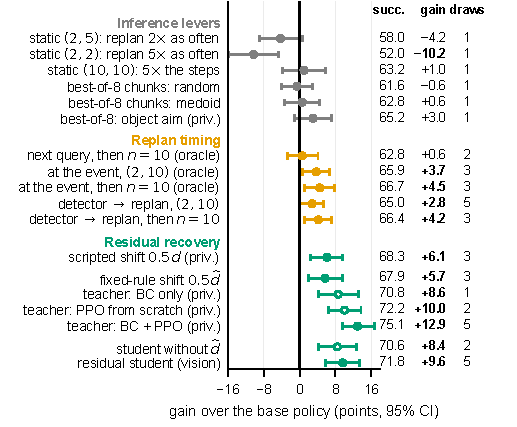
\includegraphics[width=\columnwidth]{figures/res_forest.pdf}
\caption{Gain on the 250 disturbed episodes from held-out initial states over the base policy
$(2,10)$ (mean of seven noise draws, 62.2\%); task-stratified paired
bootstrap 95\% intervals. $(n,h)$: integration steps and executed actions per query; ``oracle'': event time from the simulator; ``priv.'': uses simulator state; ``static'': fixed
schedule; hollow: ablations. Right: success, gain (bold when the interval
excludes zero), noise draws.}
\label{fig:forest}
\end{figure}

\subsection{Inference Levers Recover Little}\label{sec:levers}
Fig.~\ref{fig:forest} (top, held out) shows fixed settings of the levers that adaptive-inference methods tune, not those methods themselves. Replanning twice as often, $(2,5)$, trends down
($-4.2$) and five times as often, $(2,2)$, loses ten points (87.9\% undisturbed), and every schedule tested falls 29--33 points below its own undisturbed success (all 500). Five times more integration steps, $(10,10)$, change nothing measurable ($+1.0$). Selecting one of $K=8$ sampled chunks for the seven queries after the (oracle-timed) event also recovers little: random $-0.6$, medoid $+0.6$, a privileged rule aiming at the displaced object $+3.0$. 


\subsection{When to Replan: At the Event}\label{sec:event}
The base policy already replans at the next scheduled query. On held-out episodes, spending $n=10$ steps on that query and up to two more (oracle event timing) gains nothing measurable ($+0.6$ [$-2.6$, $+4.1$]), whereas, with the same oracle, moving the query \emph{to} the displacement gains $+3.7$ at $(2,10)$ and $+4.5$ with $n=10$ on the three queries from it, the latter $+3.9$ [$+0.4$, $+7.3$] above the next-query variant. The learned detector realizes most of this without the
oracle ($+2.8$ and $+4.2$; all 500: Table~\ref{tab:rec}) at $1.00\times$ and $1.02\times$ the policy-query time. In closed loop it detects 87--90\% of the displacements on held-out initial states within three control steps (98--100\% on training states), with 0.10--0.15 false alarms per disturbed episode, and leaves undisturbed success at
95.2\% on all 500 (base 95.4\% at the same noise, 95.1\% over three draws).

\subsection{How Much to Correct: Residual Recovery}\label{sec:correct}
 On held-out episodes the privileged scripted shift and the fixed-rule shift by $0.5\,\hat d$, which adds a replan at each detection, gain about the same ($+6.1$ and $+5.7$, three draws each; Fig.~\ref{fig:forest}). With privileged $d$, the detector's replan plus the scripted shift reaches 71.3\% held out (three draws), $+6.4$ [$+2.9$, $+10.1$] above the replan alone: shifting the actions adds to replanning. Learning the correction
helps further: the privileged teacher, whose correction is longer and more gradual than the scripted shift's, reaches 75.1\% on held-out
episodes ($+12.9$ [$+9.5$, $+16.6$], five draws), $+4.3$ [$+0.5$, $+8.4$]
above its behavior-cloned start (70.8\%, one draw); PPO from scratch reaches 72.2\% (two draws), 2.9 points [$-0.4$, $+6.3$] below the teacher. We did not distill a student from the behavior-cloned start, so PPO's share of the student's gain is not measured.

The distilled student comes within a few points of its teacher
without any privileged input: 71.8\% held out ($+9.6$ [$+5.8$, $+13.4$], five draws;
$-4.4$ [$-7.3$, $-1.6$] against the teacher with the same replan) and
75.9\% on all 500 episodes (Table~\ref{tab:rec}; 75.9--76.8\% over three distillation seeds). Held out, it is $+3.9$ [$+0.9$, $+6.9$] above the fixed-rule shift and $+3.9$ [$+1.2$, $+6.8$] above the rule selected on training initial states among seven settings ($\alpha=0.5$ over $k=4$ queries, three draws; all 500: $+4.7$ and $+4.8$). On undisturbed episodes the
student (active in 5\% through false alarms) scores 95.4\%, as does the base draw with the same noise (one episode flips each way); against three base draws it is $+0.3$ [$-1.0$, $+1.7$], so the 95\% interval excludes drops above about one point. Against the 32.6\,ms GPU policy query, the detector takes 0.4\,ms per control step, the regressor 2.2\,ms per detection and the student MLP 0.02\,ms per active query (two CPU threads; full loop not timed).

\begin{table}[t]
\caption{Recovery on 500 Disturbed and on Undisturbed Episodes (Bold: Vision-Only Student)}
\label{tab:rec}
\centering
\scriptsize
\setlength{\tabcolsep}{2.1pt}
\begin{tabular}{llcccc}
\toprule
Method & In. & Draws & Succ. & Gain [95\% interval] & Undist. \\
\midrule
$\pi_{0.5}$ alone, $(2,10)$ & -- & 7 & 64.7 & -- & 95.4 \\
Detector $\rightarrow$ replan, $(2,10)$ & V & 5 & 67.2 & $+2.5$ [$+0.6$, $+4.5$] & 95.2 \\
Detector $\rightarrow$ replan, then $n{=}10$ & V & 3 & 67.9 & $+3.3$ [$+1.0$, $+5.5$] & -- \\
Scripted shift $0.5\,d$ & P & 3 & 70.9 & $+6.3$ [$+3.9$, $+8.7$] & 90.8 \\
Fixed-rule shift, $0.5\,\hat d$ & V & 3 & 71.2 & $+6.5$ [$+3.7$, $+9.3$] & 95.4 \\
Residual teacher (BC + PPO) & P & 5 & 77.4 & $+12.7$ [$+10.1$, $+15.3$] & 95.2 \\
Student without $\hat d$ & V & 2 & 74.5 & $+9.8$ [$+6.9$, $+12.7$] & 95.4 \\
\textbf{Residual student} & V & 5 & \textbf{75.9} & $\mathbf{+11.2}$ [$+8.5$, $+13.9$] & 95.4 \\
\bottomrule
\multicolumn{6}{l}{\scriptsize In.: V vision + proprioception, P privileged state. Succ.: mean over draws;} \\
\multicolumn{6}{l}{\scriptsize half of the 500 episodes use training initial states. Undist.: one draw, with} \\
\multicolumn{6}{l}{\scriptsize the base row's sampling-noise seed (base over three draws: 95.1).}
\end{tabular}
\end{table}

\subsection{Other Disturbances and Side Effects}
The student and detector were trained only on 4--6\,cm displacements, mostly during the approach (the regressor on 2--10\,cm); Fig.~\ref{fig:general} evaluates them unchanged on other disturbances (all 500 episodes). With 8--12\,cm displacements, where the base policy falls to 37.0\% (three draws), the student gains $+8.3$ [$+5.0$, $+11.5$] and the privileged teacher $+12.1$ (two draws each; $+5.8$ to $+8.8$ over three student seeds), while the fixed-rule shift gains only $+3.8$ (three draws). The student is $+4.5$ [$+1.5$, $+7.5$] above it ($+4.2$ above the selected rule, two draws). Beyond the regressor's 10\,cm training range the student still gains $+8.0$ [$+3.7$, $+12.4$] ($+7.7$ [$+1.9$, $+13.6$] on held-out initial states). On the other disturbances the student is neutral: for a late move of the nearest free object
(steps 100--200) the detector fires in half of the episodes and the student's gain is within noise ($+1.4$), whereas the privileged teacher is slightly harmful ($-2.4$ [$-4.2$, $-0.5$], two draws each); for sliding (6--10\,cm planned, cut short when the gripper closes, so realized slides differ by method) and a five-step arm push the detector, trained on teleports, rarely fires (6--12\%) and success
changes by at most 1.1 points. Undisturbed success is 95.2--95.6\% in every detector-gated variant measured: the detector gate bounds how often a residual can act, whereas the scripted shift's cumulative gate costs 4.6 points (90.8\%).

\begin{figure}[t]
\centering
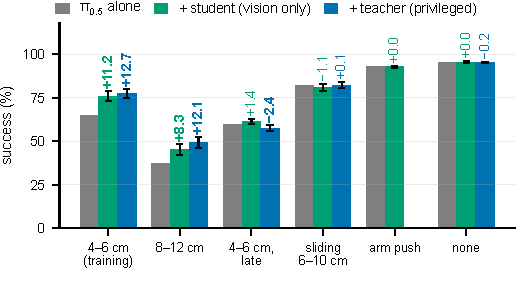
\includegraphics[width=\columnwidth]{figures/res_general.pdf}
\caption{Gains under the training disturbance (left), other disturbances and ``none'' (500 episodes each; draws, baseline/methods: 7/5 at 4--6\,cm, 3/2 at 8--12\,cm, 2/2 late, 2/1 sliding, 1/1 otherwise; the teacher was not run with the arm push). Paired gains with 95\%
intervals, bold when excluding zero. }
\label{fig:general}
\end{figure}

\begin{figure}[t]
\centering
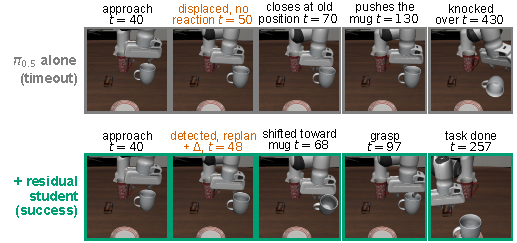
\includegraphics[width=\columnwidth]{figures/res_qual.pdf}
\caption{One episode of the mug-and-pudding task from a held-out initial state, with the same sampling noise in both rows; $t$ is the control step. Top: the base policy alone (timeout). Bottom: with the detector and residual student (success).}
\label{fig:qual}
\end{figure}

\subsection{Ablation: Displacement Estimate}
A student distilled without $\hat d$ is only slightly worse than the full student on all 500 episodes ($-1.4$ [$-3.5$, $+0.9$], two draws; $-1.4$ to $-2.8$ over three distillation seeds): at 4--6\,cm the detector tells it \emph{when}, while the base chunk, proprioception and the task input may tell it \emph{how}. At 8--12\,cm $\hat d$ helps in two of three seeds (without it: $-3.9$ [$-6.5$, $-1.3$], two draws; other seeds $-6.0$ and $+0.8$). It does not make the correction proportional: held out, from 4--6 to 8--12\,cm displacements the student's shift along the displacement grows only from 2.3 to 3.2\,cm (the teacher's from 3.3 to 9.2\,cm), as the regressor saturates near 6\,cm.

\subsection{Where the Residual Helps and Where It Fails}
Gains concentrate where the approach triggers the event: held out, the student gains $+12.3$ [$+7.6$, $+17.1$] on the 179 approach-triggered episodes but $+2.7$ [$-2.6$, $+7.9$] on the 71 where the time fallback moves an object before the gripper nears it; there the privileged teacher still gains $+8.1$ and the detector's replan alone $-1.8$. The residual was active in 91\% of the student's remaining failures (85\% held out), so few are due to missed detections; the correction itself, labeled zero where the teacher's gate stayed closed, is a likely bottleneck.



In Fig.~\ref{fig:qual} the mug is displaced 5.1\,cm at $t=47$; the policy alone closes the gripper at the old position and knocks the mug over, whereas with the detector and student a new chunk arrives one step later and the mug is grasped at $t=97$. Although $\hat d$ is poor (1\,cm, wrong direction), the correction points toward the mug, so it may come from the base chunk or a task-level push.


% =====================================================================
\section{Conclusion}
% =====================================================================

When the object it approaches is suddenly displaced, $\pi_{0.5}$ often first closes the gripper
nearer its old position and loses 31 points. Replanning at the detected event recovers about three points, a
fixed-rule shift about six, and an event-gated residual (cloned, refined with RL, distilled to vision) about ten (held-out initial states) to eleven (all 500). The gate keeps this cheap post-training conservative: undisturbed success shows no measurable change, whereas a loosely gated teacher cut it to 73.6\% on held-out states. Limitations are one policy, benchmark and task set, teleports, synchronous simulation, mostly single training runs, PPO's share measured only for the teacher, and held-out states reused for model selection. Next, we test whether the correction tracks the displacement or acts partly as a task-level push, compare it with fine-tuning, and add physical disturbances, asynchronous execution, an end-to-end gate, possibly multi-agent~\cite{shin2024mars}, and hardware.

\bibliographystyle{IEEEtran}
\bibliography{refs_res}

\end{document}
